%%%%%%%%%%%%%%%%%%%%%%

%%%%%%%%%%%%%%%%%%%%%%
%%% Supplementary Plots
%%%%%%%%%%%%%%%%%%%%%%
{\setbeamercolor{background canvas}{bg=toccolor}
\begin{frame}{Supplementary Plots}

\end{frame}
}


\begin{frame}
  \begin{columns}
    \begin{column}{.8\textwidth}
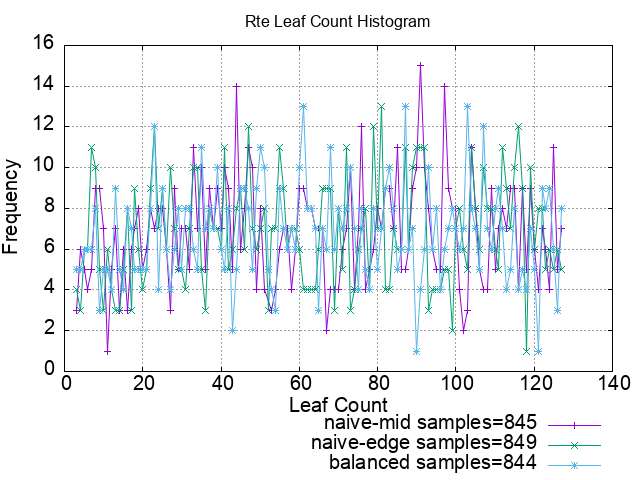
\includegraphics[width=0.9\textwidth, height=0.9\textheight, keepaspectratio]{plot-rte-leaf-count-histogram.png}
    \end{column}
    \begin{column}{.35\textwidth}
      Sampling Population.  How many RE's were generated of each leaf-count.
    \end{column}
  \end{columns}
\end{frame}


\begin{frame}
  \begin{columns}
    \begin{column}{.8\textwidth}
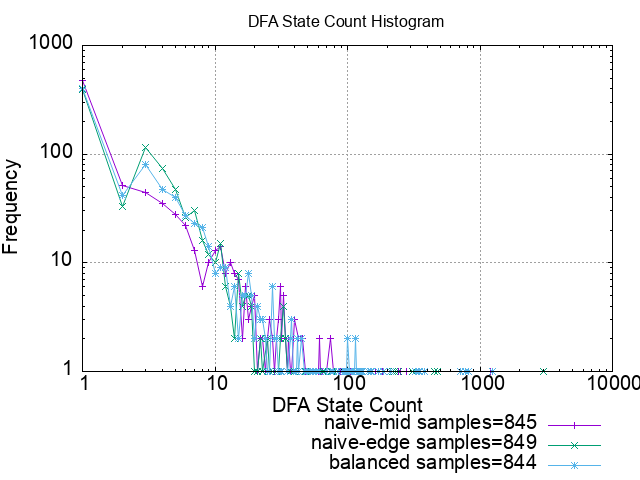
\includegraphics[width=0.9\textwidth, height=0.9\textheight, keepaspectratio]{plot-dfa-state-count-histogram.png}  
    \end{column}
    \begin{column}{.35\textwidth}
      Population Histogram of DFA state counts.
    \end{column}
  \end{columns}
\end{frame}



\begin{frame}
  \begin{columns}
    \begin{column}{.8\textwidth}
\includegraphics[width=0.9\textwidth, height=0.9\textheight, keepaspectratio]{plot-64-dfa-state-count-histogram.png}  
    \end{column}
    \begin{column}{.35\textwidth}
      \textcolor{orange}{Restricted to RTEs having exactly 64 leaf nodes.}

      \medskip
      
      Population Histogram of DFA state counts.
    \end{column}
  \end{columns}
\end{frame}

\begin{frame}
  \begin{columns}
    \begin{column}{.8\textwidth}
\includegraphics[width=0.9\textwidth, height=0.9\textheight, keepaspectratio]{plot-128-dfa-state-count-histogram.png}  
    \end{column}
    \begin{column}{.35\textwidth}
      \textcolor{orange}{Restricted to RTEs having exactly 128 leaf nodes.}

      \medskip
      
      Population Histogram of DFA state counts.
    \end{column}
  \end{columns}
\end{frame}

\begin{frame}
  \begin{columns}
    \begin{column}{.8\textwidth}
      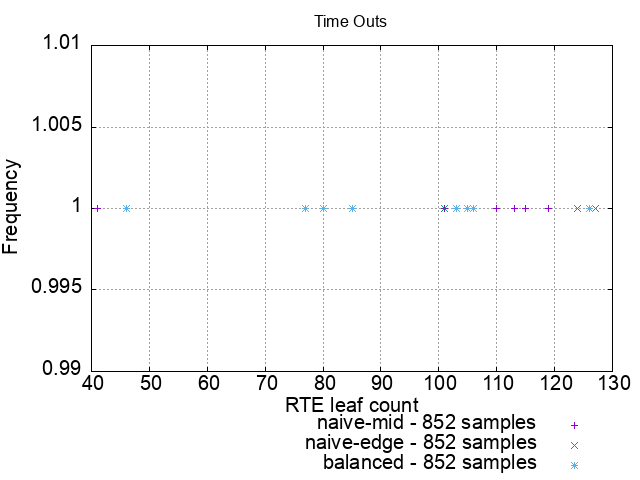
\includegraphics[width=0.9\textwidth, height=0.9\textheight, keepaspectratio]{plot-time-outs.png}
    \end{column}
    \begin{column}{.35\textwidth}
      Time-outs
    \end{column}
  \end{columns}
\end{frame}


\begin{frame}
  \begin{columns}
    \begin{column}{.8\textwidth}
\includegraphics[width=0.9\textwidth, height=0.9\textheight, keepaspectratio]{plot-average-flajolet-node-count.png}  
    \end{column}
    \begin{column}{.35\textwidth}
      Average DFA state counts vs RTE leaf counts
    \end{column}
  \end{columns}
\end{frame}

%2
\begin{frame}
  \begin{columns}
    \begin{column}{.8\textwidth}
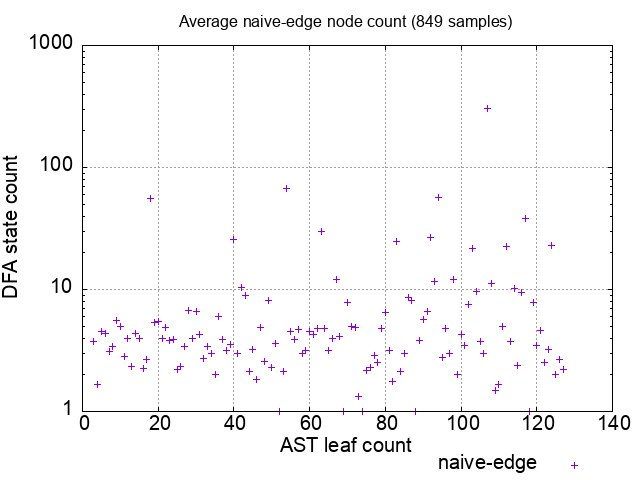
\includegraphics[width=0.9\textwidth, height=0.9\textheight, keepaspectratio]{plot-average-naive-edge-node-count.png}  
    \end{column}
    \begin{column}{.35\textwidth}
      Average DFA state counts vs RTE leaf counts
    \end{column}
  \end{columns}
\end{frame}

%3
\begin{frame}
  \begin{columns}
    \begin{column}{.8\textwidth}
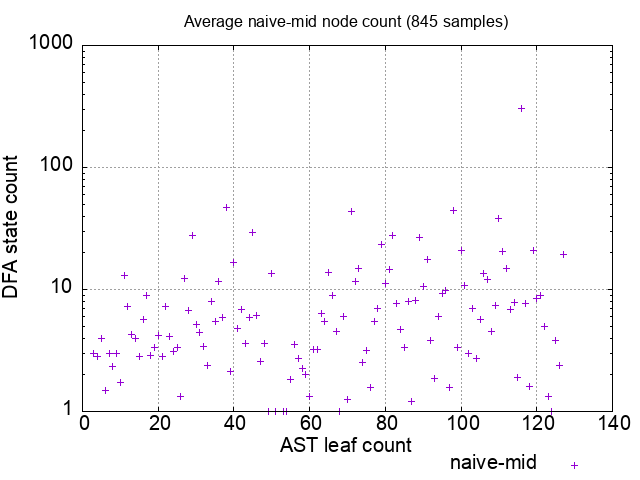
\includegraphics[width=0.9\textwidth, height=0.9\textheight, keepaspectratio]{plot-average-naive-mid-node-count.png}  
    \end{column}
    \begin{column}{.35\textwidth}
      Average DFA state counts vs RTE leaf counts
    \end{column}
  \end{columns}
\end{frame}

\begin{frame}
  \begin{columns}
    \begin{column}{.8\textwidth}
\includegraphics[width=0.9\textwidth, height=0.9\textheight, keepaspectratio]{plot-average-comb-node-count.png}  
    \end{column}
    \begin{column}{.35\textwidth}
      Average DFA state counts vs RTE leaf counts
    \end{column}
  \end{columns}
\end{frame}

%19


\begin{frame}
  \begin{columns}
    \begin{column}{.8\textwidth}
\includegraphics[width=0.9\textwidth, height=0.9\textheight, keepaspectratio]{plot-diversity.png}  
    \end{column}
    \begin{column}{.35\textwidth}
      Diversity
    \end{column}
  \end{columns}
\end{frame}




\begin{frame}
  \begin{columns}
    \begin{column}{.8\textwidth}
\includegraphics[width=0.9\textwidth, height=0.9\textheight, keepaspectratio]{plot-diversity-per-sample.png}  
    \end{column}
    \begin{column}{.35\textwidth}
      Diversity Per Sample
    \end{column}
  \end{columns}
\end{frame}








%1

%4
\begin{frame}
  \begin{columns}
    \begin{column}{.8\textwidth}
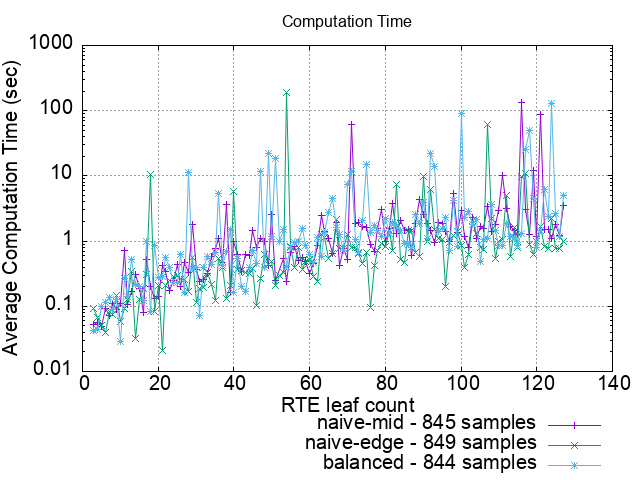
\includegraphics[width=0.9\textwidth, height=0.9\textheight, keepaspectratio]{plot-computation-time.png}  
    \end{column}
    \begin{column}{.35\textwidth}
      Computation Times per\\ RTE size (leaf count)
    \end{column}
  \end{columns}
\end{frame}

%5



%6

% use this box via:    \usebox\imbfbox
\newsavebox\imbfbox
\begin{lrbox}{\imbfbox}
  \begin{minipage}{4cm}
    \[\rho = \frac{actual~total~path~length}{ideal~total~path~length}\]

    \begin{align*}
      \rho = 1 & \implies \text{balanced}\\
      \rho < 1 & \implies \text{landscape}\\
      \rho > 1 & \implies \text{portrait}
    \end{align*}
  \end{minipage}
\end{lrbox}




%7
\begin{frame}
  \begin{columns}
    \begin{column}{.8\textwidth}
\includegraphics[width=0.9\textwidth, height=0.9\textheight, keepaspectratio]{plot-dfa-state-count-vs-Imbalance-Factor-ratsnest.png}  
    \end{column}
    \begin{column}{.35\textwidth}
      DFA state count \\vs Imbalance Factor

      \usebox\imbfbox
    \end{column}
  \end{columns}
\end{frame}



\begin{frame}
  \begin{columns}
    \begin{column}{.8\textwidth}
\includegraphics[width=0.9\textwidth, height=0.9\textheight, keepaspectratio]{plot-64-dfa-state-count-vs-Imbalance-Factor-ratsnest.png}  
    \end{column}
    \begin{column}{.35\textwidth}
      \textcolor{orange}{Restricted to RTEs having exactly 64 leaf nodes.}

      \medskip
      

      DFA state count \\vs Imbalance Factor

      \usebox\imbfbox
    \end{column}
  \end{columns}
\end{frame}

\begin{frame}
  \begin{columns}
    \begin{column}{.8\textwidth}
\includegraphics[width=0.9\textwidth, height=0.9\textheight, keepaspectratio]{plot-128-dfa-state-count-vs-Imbalance-Factor-ratsnest.png}  
    \end{column}
    \begin{column}{.35\textwidth}
      \textcolor{orange}{Restricted to RTEs having exactly 128 leaf nodes.}
      
      \medskip
      
      
      DFA state count \\vs Imbalance Factor

      \usebox\imbfbox
    \end{column}
  \end{columns}
\end{frame}

% use this box via:    \usebox\lsrbox
\newsavebox\lsrbox
\begin{lrbox}{\lsrbox}
  \begin{minipage}{4cm}
    \[\rho = \frac{longest~path}{shortest~path}\]

    \begin{align*}
      \rho = 1 & \implies \text{balanced}\\
      \rho > 1 & \implies \text{imbalanced}
    \end{align*}
  \end{minipage}
\end{lrbox}


%8
\begin{frame}
  \begin{columns}
    \begin{column}{.8\textwidth}
\includegraphics[width=0.9\textwidth, height=0.9\textheight, keepaspectratio]{plot-dfa-state-count-vs-Ratio-longest:shortest-ratsnest.png}
    \end{column}
    \begin{column}{.35\textwidth}
      DFA state count vs $\rho$

      \usebox\lsrbox
    \end{column}
  \end{columns}
\end{frame}



\begin{frame}
  \begin{columns}
    \begin{column}{.8\textwidth}
\includegraphics[width=0.9\textwidth, height=0.9\textheight, keepaspectratio]{plot-64-dfa-state-count-vs-Ratio-longest:shortest-ratsnest.png}
    \end{column}
    \begin{column}{.35\textwidth}
      \textcolor{orange}{Restricted to RTEs having exactly 64 leaf nodes.}
      
      \medskip
      
      
      DFA state count vs $\rho$

      \usebox\lsrbox

    \end{column}
  \end{columns}
\end{frame}

\begin{frame}
  \begin{columns}
    \begin{column}{.8\textwidth}
\includegraphics[width=0.9\textwidth, height=0.9\textheight, keepaspectratio]{plot-128-dfa-state-count-vs-Ratio-longest:shortest-ratsnest.png}
    \end{column}
    \begin{column}{.35\textwidth}
      \textcolor{orange}{Restricted to RTEs having exactly 128 leaf nodes.}
      
      \medskip
      
      
      DFA state count vs $\rho$

      \usebox\lsrbox

    \end{column}
  \end{columns}
\end{frame}

%9
\begin{frame}
  \begin{columns}
    \begin{column}{.8\textwidth}
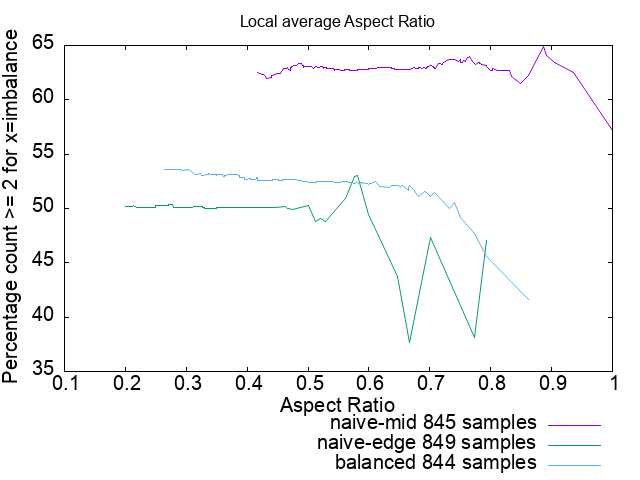
\includegraphics[width=0.9\textwidth, height=0.9\textheight, keepaspectratio]{plot-local-average.png}
    \end{column}
    \begin{column}{.35\textwidth}
    \end{column}
  \end{columns}
\end{frame}

%10


\begin{frame}
  \begin{columns}
    \begin{column}{.8\textwidth}
      \only<1>{\includegraphics[width=0.9\textwidth, height=0.9\textheight, keepaspectratio]{plot-retention-Imbalance-Factor.png}}
      \only<2>{\includegraphics[width=0.9\textwidth, height=0.9\textheight, keepaspectratio]{plot-retention-Imbalance-Factor-ratsnest.png}}
    \end{column}
    \begin{column}{.35\textwidth}

      Retention = $\rho = \frac{state~count}{node~count}$

      $\rho > 1$ is good.

    \end{column}
  \end{columns}
\end{frame}

\begin{frame}
  \begin{columns}
    \begin{column}{.8\textwidth}
      \includegraphics[width=0.9\textwidth, height=0.9\textheight, keepaspectratio]{plot-64-retention-Imbalance-Factor-ratsnest.png}
    \end{column}
    \begin{column}{.35\textwidth}
      \textcolor{orange}{Restricted to RTEs having exactly 64 leaf nodes.}

      \medskip

      Retention = $\rho = \frac{state~count}{node~count}$

      $\rho > 1$ is good.

    \end{column}
  \end{columns}
\end{frame}


%12 Aspect-Ratio
\begin{frame}
  \begin{columns}
    \begin{column}{.8\textwidth}
      \includegraphics[width=0.9\textwidth, height=0.9\textheight, keepaspectratio]{plot-running-balances-Aspect-Ratio.png}
    \end{column}
    \begin{column}{.33\textwidth}
      Running Balances:\\percentage of DFAs having $\geq 2$ states vs imbalance factor.

      \usebox\arbox
    \end{column}
  \end{columns}
\end{frame}



\begin{frame}
  \begin{columns}
    \begin{column}{.8\textwidth}
      \includegraphics[width=0.9\textwidth, height=0.9\textheight, keepaspectratio]{plot-64-running-balances-Aspect-Ratio.png}
    \end{column}
    \begin{column}{.33\textwidth}
      \textcolor{orange}{Limited to RTEs of exactly 64 leaf nodes}

      \medskip
      Running Balances:\\
      percentage of DFAs having $\geq 2$ states vs imbalance factor.

      \usebox\arbox
    \end{column}
  \end{columns}
\end{frame}

\begin{frame}
  \begin{columns}
    \begin{column}{.8\textwidth}
\includegraphics[width=0.9\textwidth, height=0.9\textheight, keepaspectratio]{plot-128-running-balances-Aspect-Ratio.png}
    \end{column}
    \begin{column}{.33\textwidth}
      \textcolor{orange}{Limited to RTEs of exactly 128 leaf nodes}

      \medskip
      Running Balances:\\
      percentage of DFAs having $\geq 2$ states vs imbalance factor.

      \usebox\arbox
    \end{column}
  \end{columns}
\end{frame}

%12 Imbalance-Factor
\begin{frame}
  \begin{columns}
    \begin{column}{.8\textwidth}
\includegraphics[width=0.9\textwidth, height=0.9\textheight, keepaspectratio]{plot-running-balances-Imbalance-Factor.png}
    \end{column}
    \begin{column}{.33\textwidth}
      Running Balances:\\percentage of DFAs having $\geq 2$ states vs imbalance factor.

      \medskip

      For each imbalance factor $<1 \implies \text{landscape}$ $>1 \implies\text{portrait}$
      
      \usebox\imbfbox
    \end{column}
  \end{columns}
\end{frame}



\begin{frame}
  \begin{columns}
    \begin{column}{.8\textwidth}
      \includegraphics[width=0.9\textwidth, height=0.9\textheight, keepaspectratio]{plot-64-running-balances-Imbalance-Factor.png}
    \end{column}
    \begin{column}{.33\textwidth}
      \textcolor{orange}{Limited to RTEs of exactly 64 leaf nodes}

      \medskip
      Running Balances:\\
      percentage of DFAs having $\geq 2$ states vs imbalance factor.

      \usebox\imbfbox
    \end{column}
  \end{columns}
\end{frame}

\begin{frame}
  \begin{columns}
    \begin{column}{.8\textwidth}
\includegraphics[width=0.9\textwidth, height=0.9\textheight, keepaspectratio]{plot-128-running-balances-Imbalance-Factor.png}
    \end{column}
    \begin{column}{.33\textwidth}
      \textcolor{orange}{Limited to RTEs of exactly 128 leaf nodes}

      \medskip
      Running Balances:\\
      percentage of DFAs having $\geq 2$ states vs imbalance factor.

      \medskip

      For each imbalance factor $<1 \implies \text{landscape}$ $>1 \implies\text{portrait}$
      
    \end{column}
  \end{columns}
\end{frame}

%12 Ratio-longest:shortest
\begin{frame}
  \begin{columns}
    \begin{column}{.8\textwidth}
\includegraphics[width=0.9\textwidth, height=0.9\textheight, keepaspectratio]{plot-running-balances-Ratio-longest:shortest.png}
    \end{column}
    \begin{column}{.33\textwidth}
      Running Balances:\\percentage of DFAs having $\geq 2$ states vs imbalance factor.

      \usebox\lsrbox
    \end{column}
  \end{columns}
\end{frame}



\begin{frame}
  \begin{columns}
    \begin{column}{.8\textwidth}
      \includegraphics[width=0.9\textwidth, height=0.9\textheight, keepaspectratio]{plot-64-running-balances-Ratio-longest:shortest.png}
    \end{column}
    \begin{column}{.33\textwidth}
      \textcolor{orange}{Limited to RTEs of exactly 64 leaf nodes}

      \medskip
      Running Balances:\\
      percentage of DFAs having $\geq 2$ states vs $\rho$

      \usebox\lsrbox
    \end{column}
  \end{columns}
\end{frame}

\begin{frame}
  \begin{columns}
    \begin{column}{.8\textwidth}
\includegraphics[width=0.9\textwidth, height=0.9\textheight, keepaspectratio]{plot-128-running-balances-Ratio-longest:shortest.png}
    \end{column}
    \begin{column}{.33\textwidth}
      \textcolor{orange}{Limited to RTEs of exactly 128 leaf nodes}

      \medskip
      Running Balances:\\
      percentage of DFAs having $\geq 2$ states vs $\rho$

      \usebox\lsrbox
    \end{column}
  \end{columns}
\end{frame}

%13
\begin{frame}
  \begin{columns}
    \begin{column}{.8\textwidth}
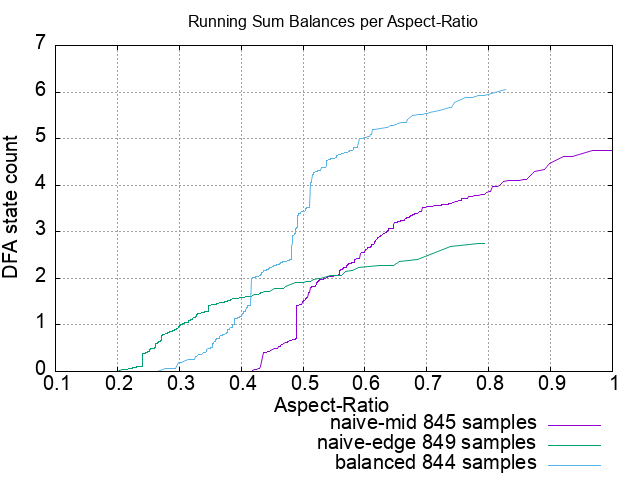
\includegraphics[width=0.9\textwidth, height=0.9\textheight, keepaspectratio]{plot-running-sum-balances-per-Aspect-Ratio.png}
    \end{column}
    \begin{column}{.35\textwidth}
      \usebox\arbox
    \end{column}
  \end{columns}
\end{frame}



\begin{frame}
  \begin{columns}
    \begin{column}{.8\textwidth}
\includegraphics[width=0.9\textwidth, height=0.9\textheight, keepaspectratio]{plot-64-running-sum-balances-per-Aspect-Ratio.png}
    \end{column}
    \begin{column}{.35\textwidth}
      \textcolor{orange}{Restricted to RTEs with exactly 64 leaf nodes}

      \usebox\arbox
    \end{column}
  \end{columns}
\end{frame}

\begin{frame}
  \begin{columns}
    \begin{column}{.8\textwidth}
\includegraphics[width=0.9\textwidth, height=0.9\textheight, keepaspectratio]{plot-128-running-sum-balances-per-Aspect-Ratio.png}
    \end{column}
    \begin{column}{.35\textwidth}
      \textcolor{orange}{Restricted to RTEs with exactly 128 leaf nodes}


      \usebox\arbox
    \end{column}
  \end{columns}
\end{frame}

%15
\begin{frame}
  \begin{columns}
    \begin{column}{.8\textwidth}
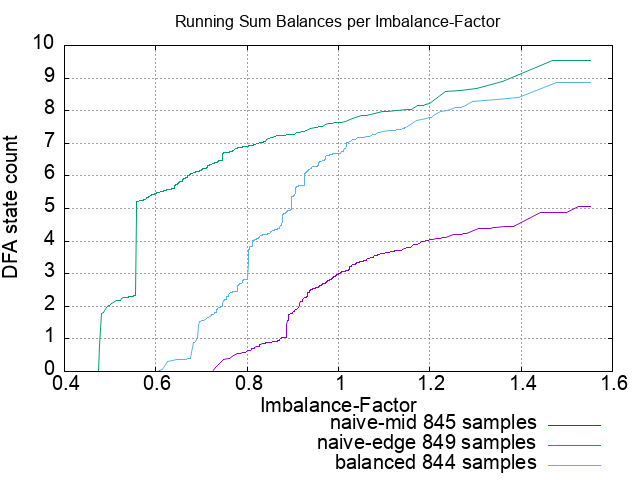
\includegraphics[width=0.9\textwidth, height=0.9\textheight, keepaspectratio]{plot-running-sum-balances-per-Imbalance-Factor.png}
    \end{column}
    \begin{column}{.35\textwidth}
      
      \usebox\imbfbox

    \end{column}
  \end{columns}
\end{frame}



\begin{frame}
  \begin{columns}
    \begin{column}{.8\textwidth}
\includegraphics[width=0.9\textwidth, height=0.9\textheight, keepaspectratio]{plot-64-running-sum-balances-per-Imbalance-Factor.png}
    \end{column}
    \begin{column}{.35\textwidth}
      \textcolor{orange}{Restricted to RTEs with exactly 64 leaf nodes}

      
      $\rho = 1 \to \text{perfectly balanced}$

      \usebox\imbfbox
    \end{column}
  \end{columns}
\end{frame}

\begin{frame}
  \begin{columns}
    \begin{column}{.8\textwidth}
\includegraphics[width=0.9\textwidth, height=0.9\textheight, keepaspectratio]{plot-128-running-sum-balances-per-Imbalance-Factor.png}
    \end{column}
    \begin{column}{.35\textwidth}
      \textcolor{orange}{Restricted to RTEs with exactly 128 leaf nodes}


      \usebox\imbfbox
    \end{column}
  \end{columns}
\end{frame}

%16
\begin{frame}
  \begin{columns}
    \begin{column}{.8\textwidth}
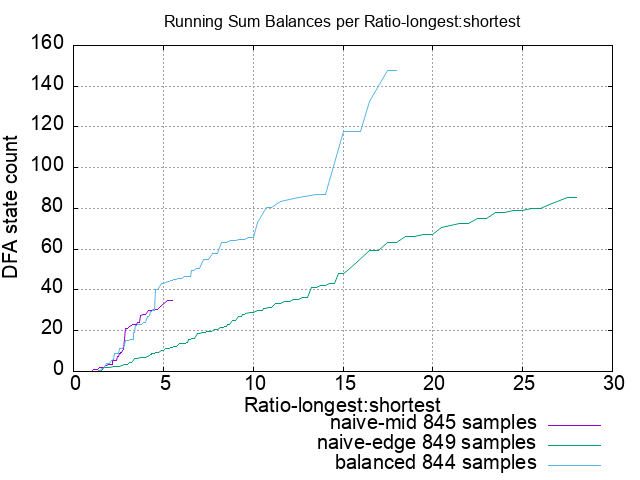
\includegraphics[width=0.9\textwidth, height=0.9\textheight, keepaspectratio]{plot-running-sum-balances-per-Ratio-longest:shortest.png}
    \end{column}
    \begin{column}{.35\textwidth}
      \usebox\lsrbox
    \end{column}
  \end{columns}
\end{frame}



\begin{frame}
  \begin{columns}
    \begin{column}{.8\textwidth}
\includegraphics[width=0.9\textwidth, height=0.9\textheight, keepaspectratio]{plot-64-running-sum-balances-per-Ratio-longest:shortest.png}
    \end{column}
    \begin{column}{.35\textwidth}
      \textcolor{orange}{Restricted to RTEs with exactly 64 leaf nodes}


      \usebox\lsrbox
    \end{column}
  \end{columns}
\end{frame}

\begin{frame}
  \begin{columns}
    \begin{column}{.8\textwidth}
\includegraphics[width=0.9\textwidth, height=0.9\textheight, keepaspectratio]{plot-128-running-sum-balances-per-Ratio-longest:shortest.png}
    \end{column}
    \begin{column}{.35\textwidth}
      \textcolor{orange}{Restricted to RTEs with exactly 128 leaf nodes}

      \usebox\lsrbox
    \end{column}
  \end{columns}
\end{frame}

%17
